\chapter{基于内存压力的自动卸载框架}
\label{chap:基于内存压力的自动卸载框架}
在\ref{chap:基于同步内存回收的内存压力量化算法的设计与实现}中,已将同步内存回收量化为内存压力。基于量化的压力值,用户态的内存压力感知卸载框架可以主动将冷页面卸载到异构后端。本章将介绍基于proc文件系统的mpfs实现、基于内存压力的工作集估计算法以及基于访问距离的匿名页和文件页的平衡算法。


\section{内存压力文件系统的实现}
\label{sec:mpfs_implementation}

基于\ref{sec:基于同步回收延迟的内存压力量化实现}章节实现的内存压力量化模型,本节构建用户态调控接口以实现冷页面的动态卸载机制。选择用户态实现方案可有效提升策略迭代效率,同时支持基于 QoS 需求的差异化策略配置。

\subsection{proc 文件系统架构分析}

proc 文件系统作为内核与用户态间的标准交互接口,其设计具有以下核心特征:

\begin{itemize}
    \item \textbf{动态生成机制:} 文件节点根据内核运行时状态实时构建
    \item \textbf{虚拟存储特性:} 不占用物理存储空间,通过内存映射实现数据存取
    \item \textbf{双向交互能力:} 支持通过标准I/O系统调用进行内核参数查询与配置
    \item \textbf{抽象访问层:} 对用户态程序隐藏内核数据结构复杂性,提供统一访问范式
\end{itemize}

上述特性使其成为实现跨态内存压力交互的理想媒介。

\subsection{mpfs 系统架构设计}

本系统通过设计内存压力文件系统(Memory Pressure File System, mpfs)实现以下核心功能:

\begin{itemize}
    \item \texttt{/proc/mpfs/mem\_pressure}:提供实时内存压力值轮询接口,支持事件驱动通知机制
    \item \texttt{/proc/mpfs/period}:实现采样周期动态可配置接口(时间单位:秒)
    \item \texttt{/proc/mpfs/mthreshold}:设置压力阈值触发条件(百分比形式)
\end{itemize}

表 \ref{tab:mpfs_files} 详细描述了各文件接口的操作语义及功能映射关系。

\begin{table}[H]
    \centering
    \caption{mpfs 文件系统接口规范}
    \label{tab:mpfs_files}
    \begin{tabular}{lccc}
        \toprule
        \textbf{操作类型} & \texttt{mem\_pressure} & \texttt{period} & \texttt{mthreshold} \\
        \midrule
        \texttt{read} & 读取当前压力值 & 获取采样周期 & 查询当前阈值 \\
        \texttt{write} & - & 更新采样周期 & 修改触发阈值 \\
        \texttt{poll} & 事件通知机制 & - & - \\
        \bottomrule
    \end{tabular}
\end{table}

\subsection{内核模块实现细节}

系统通过注册内核模块实现功能组件,核心流程如下:

\begin{itemize}
    \item \textbf{模块初始化:} 通过 \texttt{proc\_create} 在 \texttt{/proc/mpfs} 目录下创建三个虚拟文件节点,分别绑定对应的文件操作函数集(\texttt{file\_operations})
  
    \item \textbf{压力值读取:}
    \begin{itemize}
        \item \texttt{mempressure\_read} 函数从原子变量 \texttt{current\_usage\_percent} 获取压力值
        \item 采用 \texttt{sprintf} 格式化输出保证数据可读性
    \end{itemize}

    \item \textbf{事件通知机制:}
    \begin{itemize}
        \item \texttt{mempressure\_poll} 将进程加入等待队列 \texttt{mem\_waitq}
        \item 当工作队列计算出压力值后,如果超出了阈值,将唤醒等待队列 \texttt{mem\_waitq} 上的所有进程
        \item 当 \texttt{pressure\_flag} 置位时返回 \texttt{POLLIN | POLLRDNORM} 状态码
    \end{itemize}

    \item \textbf{参数动态配置:}
    \begin{itemize}
        \item 采样周期更新函数 \texttt{mempressure\_period\_write} 包含整型参数校验逻辑
        \item 阈值修改函数 \texttt{mempressure\_threshold\_write} 实施百分比有效性验证
    \end{itemize}
\end{itemize}

该架构通过标准文件接口实现用户态策略与控制参数的动态注入,同时保证内核态监测机制的实时响应能力。




\section{基于内存压力的动态调控模型}
\label{sec:pressure_based_model}

传统工作集估计方法依赖内核态时间、应用吞吐量变化率、回收事件计数器等间接指标,其有效性受限于运维人员对存储硬件特性与内核行为的专业认知。在\ref{chap:基于同步内存回收的内存压力量化算法的设计与实现}中,本研究提出基于同步内存回收的压力指标,可以自适应不同的负载和异构卸载后端。本节我们就基于定义的内存压力,来实现基于内存压力的动态调控。此模型采用主动回收策略,通过监控系统内存压力来维持目标压力区间,并将低访问频率数据页迁移至基于`frontswap`的异构存储后端,从而实现内存利用率的优化。

\begin{figure}[h]
\centering
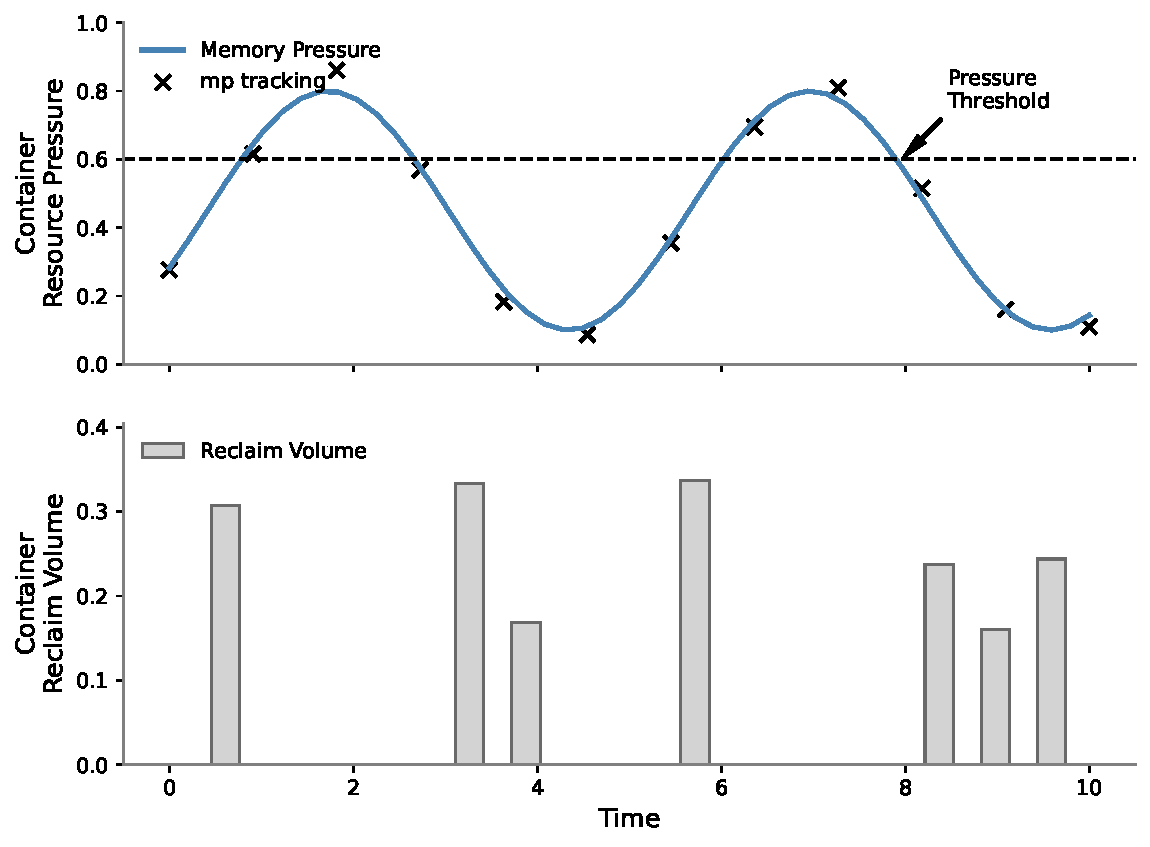
\includegraphics[width=0.95\textwidth]{压力与回收.pdf}
\caption{内存压力与页面回收调控机制}
\label{fig:pressure_work_set}
\end{figure}

本算法通过压力量化与反馈机制来实现内存的动态调控。不同于传统的静态内存管理策略,本算法根据系统的实时内存压力调整内存的使用范围,确保系统在高负载时能够扩展内存资源,在低负载时又能将冷页面主动卸载。这种基于内存压力的调控方法能够有效应对突发负载变化,并在保证系统稳定性的同时,提高内存资源的利用率。

图\ref{fig:pressure_work_set}展示了本模型的设计目标,即通过监控系统的内存压力,采用动态调整策略,确保系统内存处于合理的使用范围内。具体而言,当系统内存压力超过设定目标时,系统会逐步放宽内存限制;反之,内存压力较低时,系统会收紧内存限制。这样,不仅能在高负载时避免内存不足的问题,还能在低负载时将冷页面主动卸载。

本算法采用压力积分反馈机制,其中的关键参数体系如表\ref{tab:params}所示。算法每6秒钟执行一次,设定一个目标内存压力阈值,实现系统的平滑调节。累积的压力误差是通过比较实际内存压力与目标内存压力阈值的差异来计算的,从而形成一个时间窗口内的压力累积效应。



\begin{table}[H]
\centering
\caption{调控参数体系}
\label{tab:params}
\begin{tabular}{cccc}
\toprule
参数 & 符号 & 默认值 & 作用域 \\
\midrule
目标压力 & \(mem\_pressure\_target\) & 0.1\% & 全局 \\
最大收缩率 & \(M_p\) & 0.01 & 缩容阶段 \\
最大扩张率 & \(M_b\) & 1.0 & 扩容阶段 \\
收缩灵敏度 & \(C_p\) & 10 & 缩容触发 \\
扩张灵敏度 & \(C_b\) & 20 & 扩容触发 \\
\bottomrule
\end{tabular}
\end{table}

\begin{algorithm}[H]
    \caption{基于压力的内存调控算法}
    \label{alg:control}
    \Input{\(mem\_pressure\), \(mem\_pressure\_target\), \(C_b\), \(C_p\), \(M_b\), \(M_p\), \(min\_size\), \(max\_size\)}
    \Output{Memory Limit \(Limit\)}
    \While{\textrm{true}}{  
        \(mem\_pressure\) get from proc file system;\\
        \If{\(mem\_pressure > mem\_pressure\_target\)}{
            % Calculate expansion coefficient eta
            \(\eta \leftarrow \min\left(\left(\frac{mem\_pressure/mem\_pressure\_target}{C_b}\right)^2, 1\right)\)*\(M_b\)\;
            % Perform expansion
            \(Limit \leftarrow \min(max\_size, Limit \times (1 + \eta))\)\;
            }
        \Else{
            % Calculate contraction coefficient eta
            \(\eta \leftarrow \min\left(\left(\frac{mem\_pressure\_target/mem\_pressure}{C_p}\right)^2, 1\right)\)*\(M_p\)\;
            % Perform contraction
            \(Limit \leftarrow \max(min\_size, Limit \times (1 - \eta))\)\;
            }
        % Apply the new memory limit
        Apply new memory limit \(Limit\)\;
    }
\end{algorithm}

\begin{itemize}
\item \textbf{灵敏度系数(\(C_p, C_b\))}: 
  \begin{itemize}
  \item 扩张灵敏度\(C_b=20\): 当累积压力超过目标值20倍时达到最大扩容比例
  \item 收缩灵敏度\(C_p=10\): 当压力低于目标值1/10时触发最大缩容
  \end{itemize}

\item \textbf{最大比例(\(M_p, M_b\))}: 
  \begin{itemize}
  \item \(M_b=1.0\)允许单次扩容100\%,应对突发压力
  \item \(M_p=0.01\)限制单次缩容1\%,确保服务稳定性
  \end{itemize}

\item \textbf{积分机制}: 
  \begin{itemize}
  \item 累积窗口\(T_{interval}=6s\)平滑瞬时波动
  \item 压力增量\(\Delta P\)累计检测持续负载
  \end{itemize}
\end{itemize}

本算法的设计考虑了内存压力的动态变化与不同负载场景下的需求,因此参数体系中包含了多种灵敏度、最大收缩比例、扩张比例等调控因子,用于灵活应对系统的负载变化。例如,扩张灵敏度\(C_b = 20\)表示当实际内存压力超过目标压力的20倍时,系统会达到最大扩容比例;收缩灵敏度\(C_p = 10\)则表示当实际内存压力低于目标压力的1/10时,系统会触发最大缩容。

最大扩张比例\(M_b = 1.0\)允许单次扩容至最大限制的100\%,应对突发的内存压力;而最大收缩比例\(M_p = 0.01\)限制单次缩容不超过1\%,确保系统的稳定性,避免因过快的收缩而导致服务质量下降。通过这些参数的调整,系统能够灵活应对不同的负载条件,避免内存资源的过度浪费,并确保在需要时能够快速扩展内存。


需要特别强调的是,上述算法只是一个示例,目的是展示如何基于内存压力进行动态调控。在实际应用中,用户可以根据不同的服务质量(QoS)要求、系统负载特性或硬件架构,单独配置这些参数,甚至根据负载类型重新定义内存调控策略。例如,在某些高实时性应用中,可能会选择较高的扩张灵敏度 \(C_b\) 和较低的收缩灵敏度 \(C_p\),以确保快速响应压力变化。而在对于一般后台任务的处理上,则可能会选用较为保守的策略,以确保稳定性和节省资源。

通过采用灵活配置的方式,本算法能够根据不同的需求调整内存压力阈值、调节因子和策略参数,从而提供更具针对性和适应性的内存管理策略。算法的灵活性使得它能够适用于不同的负载场景和硬件环境,满足各种不同应用的内存管理需求。

此外,该算法可以结合不同的内存管理机制,如基于事件驱动的非阻塞方法,避免轮询带来的性能损失。未来也可以通过引入机器学习或预测算法,自动调整调控策略和参数,以实现更加智能和自适应的内存管理。算法本身也可以与其他资源管理策略结合,共同优化系统的整体性能和资源分配。

% \section{内存压力文件系统的实现}
% \label{sec:mpfs_implementation}

% 在\ref{sec:基于同步回收延迟的内存压力量化实现}中,本研究已经实现了基于同步回收延迟的内存压力量化实现,我们需要根据压力来进行调控,实现冷页面的自动卸载。在用户态实现可以更快进行迭代,也可以根据负载的实际的QOS来设置不同的策略。

% 所以本研究需要将压力的值暴露给用户态,通过proc文件系统来实现是一个很好的方法。

% \subsubsection{proc 文件系统概述}

% proc 文件系统是一种特殊的、由内核动态生成的伪文件系统,通常挂载于 /proc 目录。它并不存储在物理磁盘上,而是存在于内存中,为用户空间提供了一种访问和修改内核信息的标准接口。proc 文件系统具有以下几个关键特性:

% \begin{itemize}
%     \item \textbf{动态性:} proc 文件系统中的文件和目录并非静态存在,而是由内核根据当前系统状态动态生成。
%     \item \textbf{虚拟性:} proc 文件系统中的文件不占用实际的磁盘空间,它们只是内核数据的虚拟表示。
%     \item \textbf{交互性:} 用户可以通过标准的文件 I/O 操作(如 \texttt{read}、\texttt{write}、\texttt{poll} 等)与 proc 文件系统中的文件进行交互,从而读取内核信息或修改内核参数。
%     \item \textbf{通用性:} proc 文件系统提供了一套统一的接口,使得用户空间的应用程序无需了解内核内部的复杂数据结构,即可方便地访问内核信息。
% \end{itemize}

% 基于 proc 文件系统的这些特性,它非常适合作为用户态与内核态之间进行信息交换的桥梁。

% \subsubsection{mpfs 的设计与实现}

% \texttt{mpfs} 的设计目标是提供一个轻量级、响应及时的接口,供用户态程序获取和监控系统的内存压力信息,并支持基于内存压力的事件通知机制。为了实现这一目标,\texttt{mpfs} 提供了以下三个文件接口:

% \begin{itemize}
%     \item \texttt{/proc/mpfs/mem\_pressure}:用于读取当前系统的内存压力值(百分比)。该文件支持 poll 系统调用,当内存压力超过预设阈值时,会触发可读事件,从而通知等待中的用户态程序。
%     \item \texttt{/proc/mpfs/period}:用于读取和设置内存压力采样周期(单位:秒)。用户态程序可以通过写入该文件来动态调整采样频率。
%     \item \texttt{/proc/mpfs/mthreshold}:用于读取和设置内存压力阈值(百分比)。当内存压力超过该阈值时,\texttt{/proc/mpfs/mem\_pressure} 文件的 poll 调用会返回可读事件。
% \end{itemize}

% 表 \ref{tab:mpfs_files} 总结了 mpfs 中各个文件接口及其对应的文件操作函数。

% \begin{table}[H]
%     \centering
%     \caption{mpfs 文件接口及操作}
%     \label{tab:mpfs_files}
%     \begin{tabular}{cccc} % 四列,都居中对齐
%         \toprule
%         \textbf{操作} & \textbf{\texttt{/proc/mpfs/mem\_pressure}} & \textbf{\texttt{/proc/mpfs/period}} & \textbf{\texttt{/proc/mpfs/mthreshold}} \\
%         \midrule
%         \texttt{read} & 获取内存压力 & 获取采样周期 & 获取压力阈值 \\
%         \texttt{write} &  & 设置采样周期 & 设置压力阈值 \\
%         \texttt{poll} & 内存压力事件通知 &  &  \\
%         \bottomrule
%     \end{tabular}
% \end{table}


% mpfs 的核心实现基于内核模块机制。在模块初始化函数 (mempressure\_init) 中,通过 proc\_create 函数创建了上述三个文件节点,并分别指定了它们的文件操作函数集(file\_operations 结构)。

% \begin{itemize}
%     \item \textbf{\texttt{mem\_pressure}} 文件:
%     \begin{itemize}
%         \item \texttt{read} 操作:调用 \texttt{mempressure\_read} 函数,从全局静态变量处获取当前内存压力值,并将其格式化为字符串后复制到用户空间缓冲区。
%         \item \texttt{poll} 操作:调用 \texttt{mempressure\_poll} 函数,该函数首先将当前进程添加到等待队列 \texttt{mem\_waitq} 中,然后调用\texttt{mempressure\_read}查看内存压力,。如果内存压力超过阈值,则返回 \texttt{POLLIN | POLLRDNORM},表示文件可读;否则,进程将进入睡眠状态,等待被唤醒。
%     \end{itemize}

% \item \textbf{\texttt{period}} 文件:
%     \begin{itemize}
%         \item \texttt{read} 操作:调用 \texttt{mempressure\_period\_read} 函数,该函数读取全局变量 \texttt{sample\_period}(采样周期,单位:秒),并将其格式化为字符串后复制到用户空间缓冲区。
%         \item \texttt{write} 操作:调用 \texttt{mempressure\_period\_write} 函数,该函数从用户空间缓冲区读取新的采样周期值,并进行合法性检查(必须为正整数)。然后更新采样周期,等到之后工作队列就可以采用新的采样周期。
%     \end{itemize}

%     \item \textbf{\texttt{mthreshold}} 文件:
%     \begin{itemize}
%     \item \texttt{read} 操作:调用 \texttt{mempressure\_threshold\_read} 函数,该函数读取全局变量 \texttt{mem\_pressure\_threshold}(内存压力阈值,百分比),并将其格式化为字符串后复制到用户空间缓冲区。
%     \item \texttt{write} 操作:调用 \texttt{mempressure\_threshold\_write} 函数,该函数从用户空间缓冲区读取新的阈值,并进行合法性检查)。然后更新阈值就可以返回。
%     \end{itemize}
% \end{itemize}

% 内存压力的周期性监测和事件通知由工作队列 \texttt{pressure\_work} 实现。工作队列的处理函数 \texttt{mempressure\_workfunc} 执行以下操作:

% \begin{enumerate}
%     \item 获取系统内存信息(总内存、可用内存),计算内存使用率(百分比)。
%     \item 将计算得到的内存使用率更新到原子变量 current\_usage\_percent。
%     \item 检查内存使用率是否超过阈值 mem\_pressure\_threshold。如果超过,则设置内存压力标志 pressure\_flag,并通过 wake\_up\_interruptible 函数唤醒等待队列 mem\_waitq 上的所有进程。
%     \item 根据当前采样周期 sample\_period 重新调度工作队列 pressure\_work。
% \end{enumerate}

% 通过上述设计和实现,mpfs 为用户态程序提供了一个简洁、高效的接口,用于实时监控系统内存压力,并根据需要调整采样周期和阈值。



\section{冷热页面优化}

\subsection{冷热页面优化算法}

\subsubsection{Linux内核中的Shrinker机制分析}

Linux内核中的Shrinker机制是内存回收子系统的重要组成部分,用于在系统内存压力增大时回收可释放的缓存对象。当系统内存不足时,页面回收进程会调用注册的shrinker回调函数来释放缓存,从而缓解内存压力。Shrinker机制主要应用于各类缓存系统,如inode缓存、dentry缓存和各种文件系统的专用缓存等。

\subsection{Shrinker机制的工作原理}

在Linux内核中,各个子系统通常会维护各自的缓存以提高性能。当系统内存紧张时,内核需要一种机制来回收这些缓存所占用的内存。Shrinker机制正是为解决这个问题而设计的,它提供了一个统一的接口,使得内存回收子系统能够对各类缓存施加回收压力。

Shrinker机制在内核的页面回收路径中起作用,特别是在以下场景:
\begin{itemize}
    \item 直接内存回收(Direct Reclaim):当分配内存失败且允许等待时触发
    \item kswapd内核线程:周期性检查内存状态,在内存压力大时主动回收
    \item 内存紧急回收(Memory Cgroup Reclaim):当某个内存控制组超出限制时触发
\end{itemize}

\subsection{核心数据结构分析}

Shrinker机制主要涉及两个关键数据结构:\texttt{struct shrinker}和\texttt{struct shrink\_control}。

\subsubsection{shrink\_control结构体}

\texttt{struct shrink\_control}用于在页面回收子系统和shrinker回调函数之间传递信息。\ref{tab:shrink_control_struct}详细说明了结构体的成员。

\begin{table}[htbp]
\label{tab:shrink_control_struct}
\centering
\begin{tabular}{ccc}
\toprule
\textbf{成员} & \textbf{类型} & \textbf{说明} \\
\midrule
gfp\_mask & gfp\_t & 当前内存分配的标志,指示分配的约束条件 \\
\midrule
nid & int & 当前正在进行内存回收的NUMA节点ID \\
\midrule
nr\_to\_scan & unsigned long & 指示scan\_objects应尝试回收的对象数量\\
\midrule
nr\_scanned & unsigned long & scan\_objects实际处理的对象数量,默认值为nr\_to\_scan \\
\midrule
memcg & struct mem\_cgroup * & 当前正在进行内存回收的memory cgroup \\
\bottomrule
\end{tabular}
\caption{shrink\_control结构体成员说明}
\end{table}

\subsubsection{shrinker结构体}

\texttt{struct shrinker}定义了一个可注册的回调函数组,用于对可回收缓存施加压力。\ref{tab:shrinker_struct}详细说明了结构体的成员。

\begin{table}[htbp]
\label{tab:shrinker_struct}
\centering
\begin{tabular}{ccc}
\toprule
\textbf{成员} & \textbf{类型} & \textbf{说明} \\
\midrule
count\_objects & 函数指针 & 返回缓存中可释放对象的数量,若无可释放对象则返回SHRINK\_EMPTY,若无法确定或应跳过则返回0 \\
\midrule
scan\_objects & 函数指针 & 扫描缓存并尝试释放项目,返回已释放对象数量,若因潜在死锁无法继续则返回SHRINK\_STOP \\
\midrule
batch & long & 回收批次大小,0表示使用默认值 \\
\midrule
seeks & int & 重新创建一个对象所需的磁盘寻道次数,影响回收优先级 \\
\midrule
flags & unsigned & shrinker能力标志,如NUMA感知、memcg感知等 \\
\midrule
list & struct list\_head & 内部使用,用于将shrinker链接到全局列表 \\
\midrule
id & int & 在memcg\_kmem配置下使用的shrinker标识符 \\
\midrule
nr\_deferred & atomic\_long\_t * & 按节点统计的待删除对象,用于延迟处理 \\
\bottomrule
\end{tabular}
\caption{shrinker结构体成员说明}
\end{table}

\subsection{Shrinker的注册与使用}

内核提供了以下API用于注册和管理shrinker:

\begin{itemize}
    \item \texttt{prealloc\_shrinker()}:预分配shrinker相关资源
    \item \texttt{register\_shrinker\_prepared()}:注册已预分配资源的shrinker
    \item \texttt{register\_shrinker()}:注册新的shrinker
    \item \texttt{unregister\_shrinker()}:注销已注册的shrinker
    \item \texttt{free\_prealloced\_shrinker()}:释放预分配的shrinker资源
\end{itemize}

\subsection{自定义Shrinker的实现方法}

要实现一个自定义的shrinker,需要完成以下步骤:

1. 定义shrinker结构体并实现必要的回调函数
2. 注册shrinker到内核
3. 在不再需要时注销shrinker

Linux内核中的Shrinker机制为各类缓存系统提供了统一的内存回收接口,是内核内存管理的重要组成部分。通过实现count\_objects和scan\_objects回调函数,各子系统可以向内存回收子系统提供可回收对象的信息,并在内存压力下主动释放这些对象。这种机制既保证了内核在内存紧张时的稳定性,又保持了各缓存系统的独立性和灵活性。
